\documentclass[preprint]{IEIE} % for review
\usepackage{graphicx}
% 참고문헌 항목 간 간격 최소화 (분량 조절)
\makeatletter
\renewcommand\@openbib@code{\setlength{\itemsep}{0pt}\setlength{\parsep}{0pt}}
\makeatother
\title{초소형 MCU를 위한 스파이킹 신경망 컴파일러와\\Conv-AvgPool-LIF 퓨전 연산자: STM32F746 실측 연구}
\author{차주형 \\ 과학기술연합대학원대학교(UST) \\ e-mail : chacha@ust.ac.kr}
\engtitle{A Spiking Neural Network Compiler and a Fused Conv-AvgPool-LIF Operator\\for Tiny Microcontrollers: Measurements on an STM32F746}
\engauthor{JooHyoung Cha \\ University of Science and Technology (UST)}
\abstract{
By adding user interface to the usual router, an improved functional router is implemented in this paper. The proposed router is developed based on the SA1110 processor, and the system contains 1 ethernet port, 2 PCMCIA slots, and 1 serial
communication port. The Emdedded Linux is adopted as an operating system, and application programs are implemented by using QT/Embedded.
}

\begin{document}
\maketitle
\makeabstract

일반적으로 PC는 다목적 시스템인데 비해 임베디드 시스템은 흔히 내장형 시스템이라고 하며 정해진 용도에 맞추어서 최적화되어 있다. 임베디드 시스템은 PC에서와는 다른 개발 플랫폼을 사용하기 때문에 많은 애로사항이 발생한다. 현재의 임베디드 환경에 사용되어지는 마이크로프로세서의 종류도 다양하며 소프트웨어 플랫폼 역시 무수히 많은 임베디드 OS가 사용된다.

본 논문에서는 기존에 개발되어서 사용되고 있는 임베디드 OS 중에서 공개 소프트웨어인 임베디드 리눅스 시스템을 이용하여 향상된 기능의 라우터를 구현한다. 임베디드 리눅스를 사용하는 장점으로는 네트워크 호환성이 뛰어나며, 크기가 작으며, 쉽게 재구성화가 가능하다는 점이다. 본 논문에서는 구현과정에 대한 자세한 기술보다는 전체적인 작업과 사용자 인터페이스 부분에 초점을 맞추어서 기술한다.

\section{배경 및 관련 연구}\label{sec:background}

\subsection{스파이킹 신경망과 rate coding}

SNN은 실수 활성값 대신 이진 스파이크 열로 정보를 전달하는 신경망이다\cite{maass1997networks}. 본 논문이 사용하는 LIF 뉴런의 이산 시간 동역학은 다음과 같다.
\begin{equation}
U[t] = \beta\, U[t-1] + I[t]
\label{eq:lif-bg}
\end{equation}
\begin{equation}
S[t] = \Theta\bigl(U[t]-\theta\bigr),\qquad U[t] \leftarrow U[t] - \theta\, S[t]
\label{eq:lif-reset}
\end{equation}
여기서 $U$는 막전위, $\beta$는 감쇠 계수, $I[t]$는 시냅스 가중 합 입력, $\theta$는 임계값, $\Theta$는 단위 계단 함수이다. 발화 시 임계값을 차감하는 감산 리셋을 사용하며, 정수 도메인 구현과 reset delay 시맨틱은 IV장에서 상술한다. rate coding은 픽셀 강도 $x\in[0,1]$을 발화 확률로 해석하여 매 타임스텝 베르누이 표본 $\Pr(X[t]{=}1)=\mathrm{clip}(\gamma x+o,\,0,\,1)$을 추출한다. 따라서 추론 1회는 네트워크 전체를 $T$회 반복 실행하는 것이며, 지연시간은 $T$에 비례한다. 이 시간축 반복이 본 논문 설정($T{=}30$)에서 지연을 지배하는 요인이다. 학습 방법으로는 스파이크의 불연속성을 서러게이트 기울기로 우회하는 직접 학습\cite{neftci2019surrogate,wu2018stbp}과 ANN-SNN 변환\cite{rueckauer2017conversion}이 대표적이며, 본 논문은 snnTorch\cite{eshraghian2023training} 기반 직접 학습을 사용한다.

\subsection{뉴로모픽 하드웨어와 TinyML 스택}

SNN의 실행 기판으로는 Loihi\cite{davies2018loihi}, TrueNorth\cite{merolla2014truenorth} 같은 전용 뉴로모픽 칩이 대표적이나\cite{roy2019towards}, 이들은 전용 실리콘의 확보를 전제로 한다. ARM 코어에서 SNN을 소프트웨어로 실행한 선례로는 SpiNNaker\cite{furber2014spinnaker}가 있으나, 이 역시 대규모 시뮬레이션을 겨냥한 전용 플랫폼을 전제로 한다. 이와 대조적으로, 범용 MCU에서 심층 신경망을 실행하는 TinyML 스택이 존재한다. TFLM은 동적 할당 없이 정적 아레나 하나로 텐서와 상태를 관리하는 인터프리터형 런타임이고\cite{david2021tflm}, CMSIS-NN은 Cortex-M의 DSP 확장(듀얼 16비트 MAC 등)을 활용하는 최적화 커널 라이브러리다\cite{lai2018cmsisnn}. 정수 전용 추론은 활성과 가중치를 정수로 표현하고 실수 배율을 고정소수점 곱과 시프트(requantize)로 대체하며\cite{jacob2018quantization}, 양자화 인지 학습(QAT)은 학습 단계에서 양자화를 시뮬레이션하여 정확도 손실을 줄인다. MCUNet\cite{lin2020mcunet}과 MLPerf Tiny\cite{banbury2021mlperftiny}가 보여주듯 이 스택은 ANN에 대해서는 성숙해 있다. 한편 연산자 퓨전은 TVM\cite{chen2018tvm} 등 딥러닝 컴파일러의 표준 최적화 기법으로, 본 논문의 Conv+AvgPool+LIF 퓨전은 이 계보를 SNN 특유의 시간축 반복 구조에 적용한 것이다.

\subsection{본 연구의 위치}

SNN 소프트웨어 생태계에서는 NIR(Neuromorphic Intermediate Representation)가 시뮬레이터와 뉴로모픽 플랫폼 간 모델 교환을 위한 중간 표현을 제시한 바 있다\cite{pedersen2024nir}. 즉 SNN을 범용 프로세서에서 소프트웨어로 실행하는 시도 자체는 존재하지만, 이미 대규모로 보급된 단일 상용 MCU 위에서 표준 TinyML 스택과 통합하고, 커널 수준의 병목을 실측으로 규명하며, 비트 정확 검증까지 수행한 연구는 찾아보기 어렵다. 실제로 이 스택은 SNN에 대해 서론에서 요약한 세 가지 갭(LIF 연산자 부재, s16 DSP fast 경로의 커버리지 제약, 퓨전 int16 가중치 미지원)을 가지며, 그 기술적 상세와 해소 과정은 III--IV장에서 기술한다.


\section{CHACHA 컴파일러}\label{sec:compiler}

CHACHA 컴파일러(CHACHA Compiler)는 snnTorch와 Brevitas로 QAT 학습된 SNN을 초소형 MCU용 정수 전용 코드로 lowering하는 모델 컴파일러다. 그림~\ref{fig:pipeline}은 전체 흐름을 보인다. PyTorch에서 학습된 모델로부터 정수 가중치와 스케일을 추출하고, 모든 스케일과 LIF 파라미터를 Q15 고정소수점으로 변환한 뒤, Conv+AvgPool 퓨전과 FC 퍼뮤트 패스를 거쳐 C 배열과 TFLite flatbuffer의 두 백엔드로 방출한다. 다만 CHACHA 컴파일러는 범용 중간 표현(IR) 기반 인프라가 아니라, QAT 학습 모델로부터 정수 파라미터를 추출$\cdot$변환하는 정수 전용 export 파이프라인과 C 배열$\cdot$TFLite flatbuffer 백엔드용 호스트 코드 생성기 2종으로 구성된 특화 컴파일러이다.

\begin{figure}[htbp]
\centering
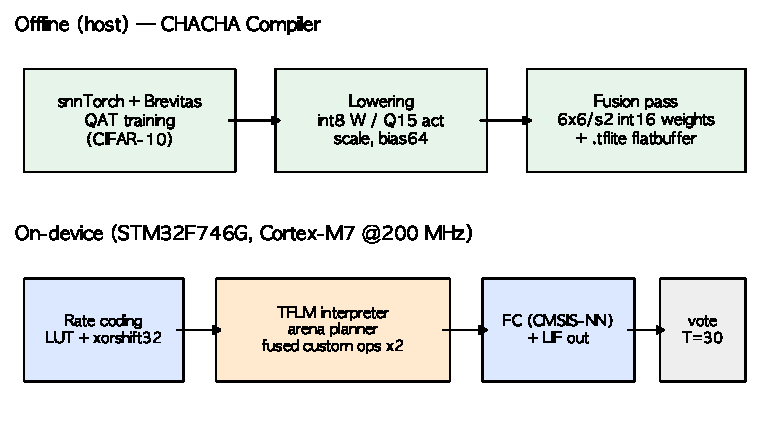
\includegraphics[width=0.9\linewidth]{figures/fig_pipeline.pdf}
\caption{CHACHA 컴파일러 전체 파이프라인. snnTorch+Brevitas QAT 학습 모델에서 정수 파라미터를 추출하고 Q15로 변환한 뒤, Conv+AvgPool 퓨전과 FC 퍼뮤트 패스를 거쳐 C 배열/TFLite flatbuffer 이중 백엔드로 방출한다.}
\label{fig:pipeline}
\end{figure}

\subsection{학습 파이프라인}\label{sec:compiler-train}

대상 모델은 LeNet-5급\cite{lecun1998gradient} SNN으로, Conv1($3\rightarrow32$, $5\times5$, 패딩 2)+AvgPool($2\times2$)+LIF1 $\rightarrow$ Conv2($32\rightarrow64$, $5\times5$, 패딩 2)+AvgPool+LIF2 $\rightarrow$ FC($4096\rightarrow10$)+LIF$_{out}$의 총 94,666 파라미터 구조다. CIFAR-10\cite{krizhevsky2009cifar}을 rate coding($T{=}30$)으로 인코딩해 입력하며, 전 레이어 공통으로 $\beta=0.9$, $\theta=1.0$을 사용한다. Conv/FC 레이어는 Brevitas\cite{brevitas2023}의 QuantConv2d/QuantLinear(\texttt{weight\_bit\_width}=8)로 구성하였고, 가중치 양자화기는 Brevitas 기본 설정을 사용하였다(per-tensor --- export 산출물의 스케일이 레이어당 스칼라 1개임을 확인). LIF는 snnTorch의 Leaky 뉴런(fast\_sigmoid 서러게이트 기울기)\cite{eshraghian2023training}이다. 학습 하이퍼파라미터와 학습 로그 정확도는 실험 재현 세부에 해당하므로 V장에서 실험 환경과 함께 기술한다. bias는 QAT 대상이 아니며 export 시 사후 양자화한다(다음 절).

\subsection{정수 전용 lowering}\label{sec:compiler-lowering}

제안 lowering의 원칙은 생성되는 C 코드에 float 타입과 리터럴을 일절 포함하지 않는 것이다. 가중치는 Brevitas의 \texttt{int\_weight()}로 int8 정수를 직접 추출하고, float 스케일 $s$는 모두 Q15 정수로 변환한다.
\begin{equation}
q = \mathrm{clip}\bigl(\mathrm{round}(s\cdot 2^{15}),\,-2^{15},\,2^{15}{-}1\bigr)
\label{eq:q15}
\end{equation}
예컨대 가중치 스케일은 conv1 $w_s{=}231$, conv2 $534$, FC $639$로, LIF 파라미터는 $\beta\rightarrow29{,}491(=\mathrm{round}(0.9\cdot2^{15}))$, $\theta\rightarrow32{,}767$(1.0의 포화값)로 방출된다. bias는 float 값을 $s_b=\max|b|/127$의 대칭 int8로 사후 양자화하고 Q15 스케일 $b_s$를 함께 방출한다.

정수 도메인 매핑은 다음과 같다. int8 가중치와 Q15 활성의 정수 누산을 $a=\sum_k w_k x_k$라 할 때, 비퓨전 기준 경로는
\begin{equation}
y_{q15} = \bigl\lfloor a\, w_s / 2^{15} \bigr\rfloor + b\, b_s
\label{eq:map-unfused}
\end{equation}
를 계산한 뒤 AvgPool이 /4 평균을 취한다(산술 시프트 절단과 풀링 반올림이 각각 발생). 퓨전 경로는 /4와 직전 층 스파이크 표현값 $s_{in}$의 보정을 하나의 실배율로 흡수한다.
\begin{equation}
M_f = \frac{w_s}{2^{15}} \cdot \frac{32767}{s_{in}} \cdot \frac{1}{4},\qquad
b_{64} = \mathrm{round}\!\left(\frac{b\, b_s}{M_f}\right)
\label{eq:mfused}
\end{equation}
출력은 $y=\mathrm{requant}(a_f+b_{64})$ 한 번으로 계산된다. 여기서 $a_f$는 퓨전 커널의 64비트 누산값이고, $M_f$는 \texttt{frexp}로 $M_f=q\cdot2^{e}$ ($q\in[0.5,1)$)로 분해되어 Q31 곱수 $m=\mathrm{round}(q\cdot2^{31})$과 시프트 $e$의 쌍으로 방출되며, 런타임은 CMSIS-NN의 64비트 requantize 루틴(\texttt{arm\_nn\_requantize\_s64})으로 이를 적용한다. 퓨전 경로는 반올림이 requantize 1회로 줄어든다. 두 경로의 수치 차이는 V장에서 분석한다(LIF1 스파이크의 0.75\%가 임계 근처에서 타이밍이 플립되나 최종 예측은 불변).

\subsection{Q15 활성 표현의 선택}\label{sec:compiler-q15}

활성값에 int8이 아닌 Q15(int16)를 사용하는 이유는 네 가지이다. 첫째, 감쇠 계수 $\beta=0.9$를 $29{,}491/32{,}768$로 표현할 수 있어 매 타임스텝 곱해지는 파라미터의 정밀도가 확보된다(int8이면 유효 정밀도가 부족하다). 둘째, 감산 리셋 후 잔여 막전위의 누적과 임계 비교에 충분한 동적 범위가 필요하다. 셋째, 스파이크를 0/32,767로 표현하면 Q15의 0/1.0에 대응한다. 넷째, Cortex-M7의 듀얼 16비트 SIMD(SMLALD, QADD16 등)가 s16 데이터를 자연스럽게 지원하므로 int8 대비 추가 비용이 없다.

\subsection{컴파일러 패스와 백엔드}\label{sec:compiler-passes}

\textbf{(1) Conv+AvgPool 퓨전 패스.} $5\times5$, 패딩 2 합성곱 뒤에 $2\times2$/스트라이드 2 평균 풀링이 이어지는 구성을 고려한다. 합성곱 출력은
\begin{equation}
c[m][n] = \sum_{u=0}^{4}\sum_{v=0}^{4} w_5[u][v]\; x[m{+}u{-}2][n{+}v{-}2]
\label{eq:conv5}
\end{equation}
이고(패딩 밖 $x$는 0), 풀링 출력은 $p[i][j]=\frac{1}{4}\sum_{dy,dx\in\{0,1\}} c[2i{+}dy][2j{+}dx]$이다. 식~(\ref{eq:conv5})를 대입하고 $a=u+dy$, $b=v+dx$로 치환하면
\begin{equation}
p[i][j] = \frac{1}{4}\sum_{a=0}^{5}\sum_{b=0}^{5} w_6[a][b]\; x[2i{+}a{-}2][2j{+}b{-}2]
\label{eq:fused6}
\end{equation}
\begin{equation}
w_6[a][b] = \sum_{dy,dx\in\{0,1\}} w_5[a{-}dy][b{-}dx]
\label{eq:w6}
\end{equation}
을 얻는다(첨자가 $[0,5)$ 범위를 벗어나는 항은 0). 즉 결과는 $2\times2$ 시프트된 $5\times5$ 커널 4개를 합친 $6\times6$ 커널을 스트라이드 2, 패딩 2로 적용한 합성곱과 같고, $1/4$은 식~(\ref{eq:mfused})의 requantize 배율 $M_f$에 흡수되므로 부동소수점 근사 없이 정수 수준에서 등가이다. bias는 네 풀링 위치에 동일하게 더해지므로 평균 후에도 변하지 않는다. 다만 $w_6$은 int8 값 4개의 합이라 $|w_6|\le508$이 되어 int8에 담기지 않으므로 int16으로 방출한다. 이것이 표준 CMSIS-NN s16 커널(int8 가중치 전용)을 사용할 수 없는 직접적 이유이며, IV장에서 커스텀 커널을 도입하는 근거가 된다. 연산량 감소와 커널 구현도 IV장에서 상술한다.

\textbf{(2) FC 퍼뮤트 패스.} 커널 출력(스파이크 텐서)은 NHWC 레이아웃인 반면 PyTorch의 FC 가중치는 CHW flatten 순서이므로, 빌드 타임에 $w'_{o,\,(8h+w)\cdot64+c}=w_{o,\,64c+8h+w}$($8\times8$ 공간, 64채널)로 재배열해 방출한다. 이로써 런타임 재배열이나 가중치의 RAM 사본이 필요 없다.

\textbf{(3) 이중 백엔드.} C 배열 백엔드는 퓨전 int16 가중치, int64 bias, (Q31 곱수, 시프트) 쌍을 const 배열(\texttt{snn\_weights\_fused.c/.h})로 방출하며 Flash에 상주시킨다. conv2 퓨전 가중치는 147,456B($\approx$147.5KB)로 SRAM(320KB)에 두기 어려워 Flash 상주가 전제된다. TFLite flatbuffer 백엔드는 커스텀 연산자를 포함한 TFLite 모델을 생성한다. 활성 텐서는 scale $1/2^{15}$, zero-point 0의 int16으로 Q15와 동일한 해석이고, 스파이크는 전 레이어 32,767로 표현한다(64비트 누산으로 오버플로가 없다 --- IV장). 퓨전 가중치 scale은 $w_s/(2^{15}\cdot4)$(평균 /4 흡수)를 CMSIS-NN 컨벤션에 따라 채널 수만큼 복제한 per-channel 배열로, bias는 입력 scale과 가중치 scale의 곱을 scale로 갖는 int64로 방출한다. 한편 C 배열 백엔드는 LIF1 출력 스파이크를 int32 누산 범위 내에서 정의된 표현인 16,384(Q14)로 나타내며, 그 보정 계수 $32767/16384$이 식~(\ref{eq:mfused})의 $M_f$에 흡수된다. 두 백엔드 모두 동일한 매핑식의 특수화이며, 생성물의 비트 정확성은 V장에서 검증한다.

현재 컴파일러가 지원하는 연산자는 본 그래프의 구성 요소(Conv, AvgPool, LIF, FC)이고, 실기기에서 검증된 모델은 본 논문의 LeNet-5급 SNN 1종이다.


\section{Conv+AvgPool+LIF 퓨전 연산자}
\label{sec:fusion}

본 장에서는 제안하는 퓨전 연산자 \texttt{SNN\_CONV\_POOL\_LIF}의 설계를
기술한다. 먼저 LIF 뉴런의 연산 시맨틱과 표준 TFLM+CMSIS-NN 경로가 본
SNN에서 성능을 잃는 구조적 원인을 분석한 뒤, 이를 해소하는 세 구성 요소
--- Conv+AvgPool 대수적 퓨전, SMLALD 기반 s16$\times$s16 커널, LIF SIMD
에필로그 --- 와 TFLite Micro(TFLM) 커스텀 연산자 통합을 차례로 설명한다.

\subsection{LIF 시맨틱과 표준 커널 경로의 한계}

LIF 뉴런의 이산 시간 동역학은 II장
식~(\ref{eq:lif-bg})--(\ref{eq:lif-reset})와 같다. 막전위 $U$는
타임스텝마다 $\beta$로 감쇠하며 시냅스 입력 $I[t]$를 누적하고, 임계값
$\theta$에 도달하면 스파이크를 발화한 뒤 막전위에서 $\theta$를 감산한다
(감산 리셋). 본 구현은 학습에 사용한 snnTorch Leaky
뉴런\cite{eshraghian2023training}의 시맨틱을 그대로 따르며, 발화한
스파이크가 다음 타임스텝에 출력되는 reset delay 시맨틱을 포함한다. 모든
활성값$\cdot$막전위$\cdot$LIF 파라미터는 Q15 int16이다($\beta=0.9$는
$29{,}491/32{,}768$).

이 모델을 표준 TinyML 스택으로 실행하면 세 가지 갭이 드러난다.

첫째, \textbf{LIF 연산자의 부재}이다. TFLM 빌트인 연산자에는 타임스텝
사이에 상태(막전위, 직전 스파이크)를 유지하는 뉴런 연산이 없으므로,
LIF는 어떤 구성에서도 커스텀 연산자로 구현해야 한다.

둘째, \textbf{CMSIS-NN s16 DSP fast 경로의 커버리지 제약}이다.
CMSIS-NN\cite{lai2018cmsisnn}의 int16 활성$\times$int8 가중치
합성곱에서 DSP 가속 경로(\texttt{arm\_convolve\_fast\_s16})는 im2col
열 길이($k_h \times k_w \times C_{in}$)가 512 미만일 때만 적용된다. 이
한계는 int16$\times$int8 곱(최대 $2^{22}$)을 int32 누산기에 오버플로
없이 누적할 수 있는 항 수가 $2^{31}/2^{22}=512$라는 데서 온다. conv1은
$5\times5\times3=75$로 조건을 만족하지만, conv2는
$5\times5\times32=800$으로 조건을 위배하여 일반 C 커널로 폴백한다.
다음 장에서 실측으로 보이듯, 이 폴백만으로 표준 경로 전체가 스칼라
구현보다 약 2.1배 느려진다.

셋째, \textbf{퓨전 int16 가중치의 미지원}이다. 아래의 Conv+AvgPool
퓨전은 int8 가중치 4개의 합을 새 가중치로 만들므로 값 범위가
$|w|\le508$이 되어 int8에 담기지 않는다. CMSIS-NN s16 커널군은 int8
가중치 전용이므로 이를 수용할 수 없다.

제안 연산자는 이 세 갭을 커스텀 커널 하나로 동시에 해소한다.

\subsection{Conv+AvgPool 대수적 퓨전}

$5\times5$/패딩 2 합성곱 뒤의 $2\times2$/스트라이드 2 평균 풀링은,
평균 풀링이 선형 연산이라는 점을 이용하여 하나의 $6\times6$/스트라이드
2/패딩 2 합성곱과 스칼라 $1/4$의 곱으로 대수적으로 결합할 수 있다.
퓨전 커널 $w_6$은 III장 식~(\ref{eq:w6})으로 빌드 타임에 생성되며,
$1/4$은 나눗셈으로 수행하지 않고 requantize 배율에 흡수하므로
--- 식~(\ref{eq:mfused}) --- 이 변환은 정수 수준에서 등가이다. 그
검증은 다음 장에서 제시한다.

퓨전의 효과는 세 가지다. (i) 타임스텝당 MAC 수가 conv1은
$2{,}457{,}600$에서 $884{,}736$으로, conv2는 $13{,}107{,}200$에서
$4{,}718{,}592$로 줄어 합성곱 합계 기준 약 2.8배 감소한다. (ii) conv 출력과 풀링 입력에 해당하는 중간 텐서가
사라져, 레이어 사이에는 스파이크 텐서($32\times16\times16$,
$64\times8\times8$)만 남는다. (iii) LIF까지 결합하면 requantize
직후의 출력 타일에 뉴런 갱신을 즉시 적용하므로 conv--pool--LIF 사이의
메모리 왕복이 완전히 제거된다. 또한 비퓨전 경로에서 두 번이던
반올림(시프트 절단, 풀링 반올림)이 requantize 한 번으로 줄어든다.
반면 가중치는 int16으로 방출되어 용량이 int8 대비 2배가 되며(conv1
$6{,}912$B, conv2 $147{,}456$B $\approx147.5$KB), conv2 퓨전 가중치는
RAM에 올리지 않고 Flash 상수로 상주시킨다. 이 용량 증가는 배포 가능
영역 분석 장에서 지배 항으로 다시 다룬다. 그림~\ref{fig:fusion}은 퓨전
전후의 연산 구조를 보인다.

\begin{figure}[htbp]
\centering
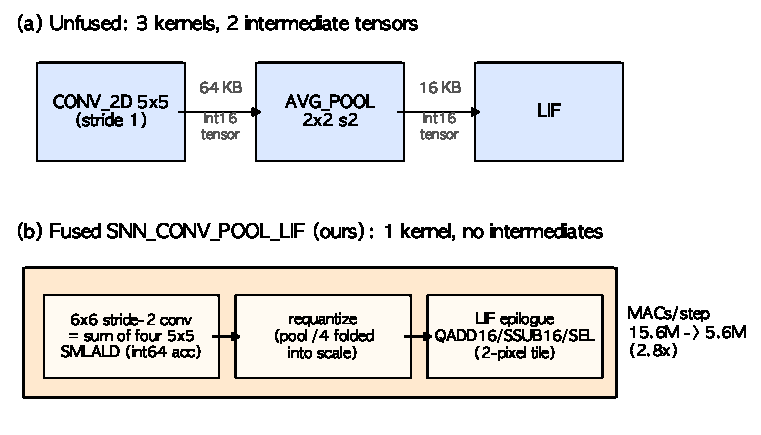
\includegraphics[width=0.9\linewidth]{figures/fig_fusion.pdf}
\caption{제안 퓨전 연산자의 구조. (a) 비퓨전 경로는 커널 3개와 중간
텐서 2개를 거친다. (b) 퓨전 경로는 $6\times6$/스트라이드 2 SMLALD
커널, requantize(풀링 $1/4$을 배율에 흡수), LIF 에필로그가 단일 커널
안에서 이어지며 중간 텐서가 없다(conv 합계 MAC 15.6M
$\rightarrow$ 5.6M/타임스텝).}
\label{fig:fusion}
\end{figure}

\subsection{SMLALD 기반 s16$\times$s16 퓨전 커널}

퓨전 가중치가 int16이므로 s16 활성$\times$s16 가중치 내적을 직접
구현하였다. im2col 구조는 CMSIS-NN
\texttt{arm\_convolve\_fast\_s16}(Apache-2.0)을 준용한다. 입력을
im2col 버퍼에 출력 픽셀 2개(2컬럼) 단위로 전개하고(패딩은 0 채움),
2컬럼이 채워지는 즉시 내적 코어에 전달하며, 홀수 출력 픽셀은 1컬럼
잔여 경로로 처리한다.

내적 코어는 im2col 2컬럼 $\times$ 출력 채널 2개를 동시에 처리하도록
누산기 4개를 유지하고, int16 두 개씩 로드하여 반복당 SMLALD를 4회
실행한다. SMLALD는 듀얼 $16\times16$ 곱을 64비트
누산기에 더하는 Cortex-M7 DSP 명령이다. 64비트 누산은 오버플로 가능성을
제거한다. 곱의 크기는 $|w|\le508<2^{9}$, $|x|\le2^{15}$에서 $2^{24}$
미만인데 conv2의 열 길이가 $6\times6\times32=1{,}152$이므로 최악 누적
합은 int32 범위를 넘지만, int64에서는 실용적인 어떤 열 길이에서도
여유가 있다. 즉 퓨전 커널에는 표준 fast 경로의 512 제약과 같은 커버리지
공백이 없다. 누산이 끝나면 채널별 $(\mathrm{mult},\mathrm{shift})$
파라미터로 \texttt{arm\_nn\_requantize\_s64}를 적용하고
$[-32{,}768,\,32{,}767]$로 클램프한다. \texttt{ARM\_MATH\_DSP}가
정의되지 않은 환경에서는 동일 산술의 스칼라 폴백으로 컴파일되며 결과는
비트 단위로 같다.

\subsection{LIF SIMD 에필로그}

requantize된 2픽셀$\times C_o$ 타일에는 LIF 갱신을 즉시 적용한다.
int16 두 레인을 한 워드에 담아 다음 4단계로 처리한다. (i)
$\beta U \gg 15$: 레인별 $16\times16$ 곱(SMULBB/SMULTB) 후 PKHBT로
재패킹, (ii) QADD16으로 입력을 레인별 포화 가산하여 $\tilde U$ 계산
--- 식~(\ref{eq:lif-bg})의 갱신, (iii) SSUB16으로 $\tilde U-\theta$를
레인별로 계산하면서 APSR.GE 플래그 설정, (iv) SEL로 분기 없이 다음
막전위(발화 레인은 $\tilde U-\theta$, 비발화 레인은 $\tilde U$)와
스파이크 값(발화 $32{,}767$, 비발화 0)을 선택한다. 출력은 직전 스텝의
스파이크를 내보내는 reset delay 시맨틱을 따른다. SIMD 경로는 관련
포인터가 모두 4바이트 정렬일 때만 진입하며, 스칼라 폴백과 비트 단위로
동일하다(전수 검증은 다음 장에서 제시).

\subsection{TFLM 커스텀 연산자 통합과 구현 제약}

제안 커널은 TFLM\cite{david2021tflm}에 커스텀 연산자
\texttt{SNN\_CONV\_POOL\_LIF1/2}와 \texttt{SNN\_LIF\_OUT}으로 등록되고,
마지막 FC 층은 빌트인 \texttt{FULLY\_CONNECTED}(CMSIS-NN int16x8)를
그대로 사용한다(\texttt{MicroMutableOpResolver}$\langle4\rangle$).
활성 텐서의 양자화는 scale $1/32{,}768$(Q15), zero point 0이며 스파이크
값은 전 레이어 $32{,}767$이다. 커널 Prepare 단계에서 채널별 유효 배율
$\mathrm{eff}=s_{in}\,s_{w}[c]/s_{out}$을 \texttt{QuantizeMultiplier}로
$(\mathrm{mult},\mathrm{shift})$에 분해한다.

메모리는 TFLM 아레나로 일원화하였다. 타임스텝을 넘어 유지되어야 하는
LIF 상태(막전위$\cdot$직전 스파이크)와 채널별 mult/shift 테이블은
\texttt{AllocatePersistentBuffer}로, Invoke 동안만 필요한 im2col
버퍼는 \texttt{RequestScratchBufferInArena}로 할당하며, 활성 텐서는
아레나 메모리 플래너가 배치한다. 그 결과 TFLM 경로의 SNN 관련 RAM은
전부 단일 아레나 안에서 관리되고 별도의 정적 배열이 없다. LIF 상태는
이미지 경계에서 재설정한다.

구현 제약은 두 가지다. batch 1 전용이며, 내부 타일이
\texttt{int16\_t tile[2*64]}로 고정되어 있어 출력 채널 수
$C_o \le 64$를 가정한다. 현 모델(32/64채널)은 이를 충족하며, 제약
완화 조건은 배포 가능 영역 분석 장에서 논의한다.


\section{실험 결과 및 검증}
\label{sec:eval}

\subsection{실험 환경과 재현성}

모든 실측은 STM32F746G-DISCO 보드(STM32F746NG: Cortex-M7 200MHz
Over-Drive, 단정밀 FPU, I/D 캐시 활성, SRAM 320KB, Flash
1MB)\cite{st_rm0385}에서 수행하였다. 툴체인은 STM32CubeIDE 내장 GNU
Tools for STM32 14.3.rel1(arm-none-eabi-gcc 14.3.1)이며, 네 변형 모두
동일하게 -O3와 LTO, \texttt{ARM\_MATH\_DSP} 조건으로 빌드하였다.
TFLM과 CMSIS-NN은 저장소에 소스로 고정(vendored)하였다 ---
CMSIS-NN은 헤더 기준 리비전 V.12.0.0(2023-09-05), TFLM은 릴리스
태그 없는 업스트림 스냅샷(TFLite 스키마 버전 3)이다.

III장의 대상 모델은 rate 기반 교차 엔트로피 손실(snnTorch
\texttt{ce\_rate\_loss})과 Adam(학습률 $2\times10^{-3}$, 배치 128,
100 에폭)으로 학습하였으며, 학습 로그 정확도는 본 장의 정확도 논의에서
보고한다.

워크로드는 CIFAR-10\cite{krizhevsky2009cifar} 이미지 1장당 rate coding
30 타임스텝($T=30$)이고, 출력 뉴런의 스파이크 값이 $16{,}000$을 넘는
타임스텝을 클래스별로 누적 투표하여 판정한다. 입력 인코딩은 V1만
newlib 표준 \texttt{rand()} 구현이고, V2--V4는 256엔트리 임계값
LUT와 xorshift32(시드 \texttt{0x12345678})를 사용하는 가속 구현이다.
시간은 \texttt{HAL\_GetTick}(해상도 1ms)으로 계측하되, 이미지 1장의
처리 루프 전체(표시 포함)를 total로, 스파이크 인코딩과 신경망 forward의
합을 NN으로 분리 기록하였다. 이미지당 2.4$\sim$9.6초가 소요되므로 1ms
해상도로 인한 상대 오차는 무시할 수 있다. RAM/Flash는 링커 맵과
ST-LINK(HOTPLUG 모드) 판독 기준이다. 변형별 평균에 사용한 이미지 수는
18/16/40/41장으로 이는 측정 세션 길이의 차이일 뿐이며, 분산 데이터는
별도로 저장하지 않았으므로 본 장은 평균값만 보고한다.

비교한 네 변형은 다음과 같다. \textbf{V1}(Scalar): 기준 CHW 스칼라
conv/pool/LIF. \textbf{V2}(TFLM+CMSIS-NN, 비퓨전):
\texttt{CONV\_2D}/\texttt{AVG\_POOL\_2D}/\texttt{FULLY\_CONNECTED}는
빌트인(CMSIS-NN int16x8) 연산자, LIF는 커스텀 SIMD 연산자, 아레나
128KB 설정. \textbf{V3}(제안): 앞 장의 \texttt{SNN\_CONV\_POOL\_LIF}
퓨전 연산자. \textbf{V4}(직접 퓨전): V3와 동일한 퓨전 커널을 TFLM 없이
직접 호출하는 구성(런타임 오버헤드 분리용). 각 변형의 연산자 구성과
아레나 설정은 본 절과 표~\ref{tab:mem}의 명세로 재구성할 수 있다.

\subsection{지연시간}

표~\ref{tab:perf}와 그림~\ref{fig:latency}, \ref{fig:timestep}에
결과를 정리하였다. 핵심 결과는 인코딩$\cdot$LIF$\cdot$런타임 조건이
동일하고 conv/pool 실행 경로만 다른 V2 대 V3 비교로, 제안 퓨전 연산자는
이미지당 $9{,}641.4$ms를 $2{,}407.0$ms로 줄여 \textbf{4.0배}
가속한다. 본 논문의 모든 배속은 이미지당 total 시간 기준이며, NN 시간
기준으로는 V3/V2가 4.10배, V3/V1이 1.89배가 된다.

주목할 실측 발견은 표준 경로의 성능 역전이다. V2는 스칼라
V1($4{,}494.2$ms)보다 오히려 약 2.1배 느리다. 원인은 IV장에서 분석한
커버리지 제약으로, 타임스텝당 MAC의 84\%를 차지하는 conv2(im2col 열
길이 800)가 s16 DSP fast 경로의 적용 조건($<512$)을 위배하여 일반 C
커널로 폴백하기 때문이다. 표준 TinyML 스택을 그대로 적용하는 것이 SNN에서는
최적화가 아니라 감속이 될 수 있음을 보여 주는 결과이다.

V3는 V1 대비로는 종단 1.87배이나, 이 수치에는 V2--V4에만 적용된 입력
인코딩 개선이 포함되므로 커널 효과만의 비교는 대 V2 기준이
공정하다(표~\ref{tab:perf} 각주). 타임스텝당 NN 시간은
147.4/319.0/77.9/77.5ms(V1/V2/V3/V4)이다. 그림~\ref{fig:timestep}에서
보듯 성능의 본질은 퓨전 커널이며, TFLM 런타임의 추가 비용은 V3와 V4의
차이인 이미지당 11.5ms, 약 0.5\%에 불과하다. 즉 해석기 기반 마이크로
런타임의 오버헤드는 SNN의 타임스텝 반복($T=30$회 Invoke)에서도 무시
가능하다.

\begin{table*}[t]
\centering
\caption{네 변형의 실측 성능 비교(이미지당, $T=30$, 동일 -O3+LTO 빌드).}
\label{tab:perf}
\footnotesize
\setlength{\tabcolsep}{4.5pt}
\begin{tabular}{l l r r r r r r}
\hline
변형 & 커널 구성 & total(ms) & NN(ms) & ms/step & 대 V2 & 대 V1 & 이미지 수 \\
\hline
V1 Scalar & 기준 CHW 스칼라, \texttt{rand()} 인코딩 & 4,494.2 & 4,422.7 & 147.4 & 2.15$\times$ & 1.00$\times$ & 18 \\
V2 TFLM+CMSIS-NN(비퓨전) & 빌트인 CONV/POOL/FC + LIF 커스텀 & 9,641.4 & 9,570.0 & 319.0 & 1.00$\times$ & 0.47$\times$ & 16 \\
V3 TFLM+퓨전(제안) & \texttt{SNN\_CONV\_POOL\_LIF} 커스텀 연산자 & \textbf{2,407.0} & 2,335.7 & 77.9 & \textbf{4.0$\times$} & 1.87$\times$ & 40 \\
V4 직접 퓨전(런타임 없음) & 동일 퓨전 커널 직접 호출 & 2,395.5 & 2,324.8 & 77.5 & 4.02$\times$ & 1.88$\times$ & 41 \\
\hline
\end{tabular}
\begin{flushleft}
\footnotesize 주: (a) 모든 배속은 total ms 기준이며, NN 기준으로는
V3/V2 $=4.10\times$, V3/V1 $=1.89\times$이다. (b) V1은 newlib
\texttt{rand()} 인코딩, V2--V4는 LUT+xorshift 인코딩이므로 대 V1
배속에는 인코딩 개선분이 포함된다. 동일 조건 비교는 대 V2이다. (c) V2
감속 원인: conv2의 im2col 열 길이 $5\times5\times32=800$이 CMSIS-NN
s16 DSP fast 경로의 적용 조건($<512$)을 위배하여 일반 C 커널로 폴백.
(d) V3$-$V4 $=$ TFLM 오버헤드 11.5ms(약 0.5\%). (e) ``이미지 수''는 각
변형의 평균 산출에 사용한 이미지 수이며, 차이는 측정 세션 길이에
기인한다.
\end{flushleft}
\end{table*}

\begin{figure}[htbp]
\centering
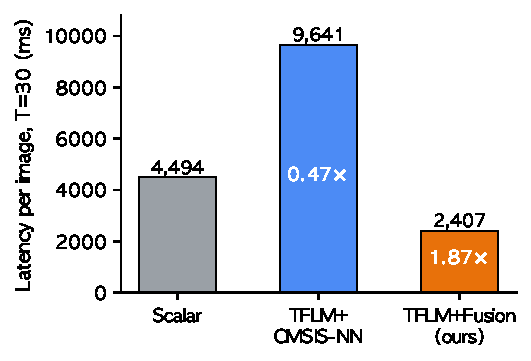
\includegraphics[width=0.86\linewidth]{figures/fig_latency.pdf}
\caption{이미지당 종단 지연시간 실측($T=30$). 막대 안의 배속은 V1
대비이다(V2 0.47$\times$, V3 1.87$\times$).}
\label{fig:latency}
\end{figure}

\begin{figure}[htbp]
\centering
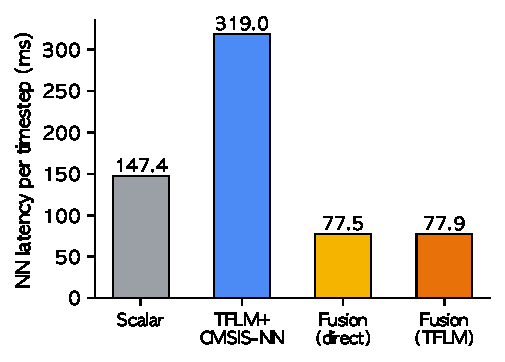
\includegraphics[width=0.86\linewidth]{figures/fig_timestep.pdf}
\caption{타임스텝당 순수 NN 시간. 직접 호출(V4)과 TFLM 통합(V3)의
차이가 TFLM 런타임 오버헤드이다(0.4ms/step, 약 0.5\%).}
\label{fig:timestep}
\end{figure}

\subsection{메모리}

표~\ref{tab:mem}과 그림~\ref{fig:memory}에 변형별 RAM/Flash를
정리하였다. 단위 표기는 본 논문 전체에서 KB는 십진(1,000B),
KiB는 이진(1,024B)이며, 표는 정확한 바이트 값을 병기한다. V3의 Flash $373{,}860$B 중 가중치 계열은
$195{,}328$B(conv1 $6{,}912$B + conv2 $147{,}456$B + FC
$40{,}960$B)이고 나머지 $178{,}532$B가 코드와 런타임이다. 이 분해는
다음 장의 가중치 예산 산술에 사용된다.

V3의 RAM $268{,}200$B는 여유 있게 설정한 256KB($262{,}144$B) 정적
아레나를 포함한 수치이며, 실제 아레나 사용량은
$80{,}288$B($\approx$80.3KB)이다. 같은 커널을 정적 버퍼로 직접
호출하는 V4의 RAM이 $85{,}512$B라는 점이 이 실사용 수치의 하한
근거이며, 아레나 설정값을 줄이면 RAM 총량도 그에 따라 줄어든다. V2는
아레나 $131{,}072$B 설정에 $84{,}544$B를 사용하였다.

\begin{table}[htbp]
\centering
\caption{변형별 메모리 사용(바이트).}
\label{tab:mem}
\footnotesize
\begin{tabular}{l r r r r}
\hline
변형 & RAM & Flash & 아레나 설정 & 아레나 실사용 \\
\hline
V1 & 251,256 & 223,556 & -- & -- \\
V2 & 186,296 & 296,052 & 131,072 & 84,544 \\
V3 & 268,200 & 373,860 & 262,144 & 80,288 \\
V4 & 85,512 & 325,168 & -- & -- \\
\hline
\end{tabular}
\begin{flushleft}
\footnotesize 주: V3의 RAM은 여유 아레나(256KB 설정)를 포함하며, SNN
실소요는 아레나 실사용 80,288B($\approx$80.3KB, 십진 KB)이다.
\end{flushleft}
\end{table}

\begin{figure}[htbp]
\centering
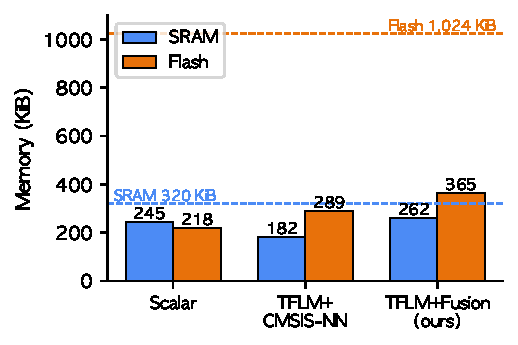
\includegraphics[width=0.86\linewidth]{figures/fig_memory.pdf}
\caption{변형별 SRAM/Flash 사용량과 보드 한계. 그림의 값은
KiB(1,024B) 단위로 본문$\cdot$표의 십진 KB와 환산 기준이 다르다(바이트
값은 표~\ref{tab:mem}). 아레나 없이 정적 버퍼를 쓰는 V4는 그림에서
제외하였다(표~\ref{tab:mem} 참조).}
\label{fig:memory}
\end{figure}

\subsection{수치 정확성 검증}

제안 경로의 정수 산술은 호스트에서 다음 네 단계로 비트 단위 검증하였다.
\begin{enumerate}
\item \textbf{퓨전 항등식}: $6\times6$ 퓨전 가중치의 raw 누산이
  $5\times5$ conv의 4위치 합과 전 픽셀$\cdot$전 채널에서 비트 일치
  --- 식~(\ref{eq:w6}) 변환의 정수 수준 등가 확인.
\item \textbf{커널 대 레퍼런스}: 퓨전 커널과 나이브 레퍼런스 구현을
  30타임스텝$\times$3가지 발화율 입력에서 비교, 스칼라 경로와 SIMD
  경로 모두 비트 일치.
\item \textbf{전체 파이프라인}: TFLM 통합 경로를 독립 레퍼런스와 비교,
  3개 테스트 케이스에서 900개의 출력 스파이크$\cdot$막전위 비트 일치,
  예측 3/3 동일.
\item \textbf{LIF SIMD 전수 검증}: LIF SIMD 커널을
  $1{,}887$만(18.87M) 입력 조합에 대해 스칼라 구현과 전수 비교하여
  비트 일치.
\end{enumerate}

기준 스칼라 경로(V1)와의 비교는 성격이 다르다. 두 경로는 반올림
위치가 다른 정수 구현으로 --- 기준 경로는 시프트 절단과 풀링 반올림의
2회, 퓨전 경로는 requantize 반올림 1회 --- 서로 비트 등가가 아니며, 이 차이로
LIF1 스파이크의 0.75\%가 임계값 근처에서 발화 타이밍이 플립된다.
호스트 3개 케이스에서 최종 예측에는 영향이 없었으며, 본 논문은 두
경로를 통계적으로 등가인 구현으로 서술한다.

\subsection{정확도 수준과 한계}

본 논문의 기여는 정확도 개선이 아니라, 주어진 QAT 모델을 비트
정확하게 그리고 빠르게 배포하는 것이다. 본 모델의 정확도 수준과 그
해석은 다음과 같다.

학습된 QAT 모델의 CIFAR-10 테스트 정확도는 학습 로그 기준으로 배포
체크포인트(에폭 96)에서 50.72\%, 학습 중 최고 51.02\%(에폭 79)였다.
이 수준은 rate coding($T=30$), $94{,}666$개 파라미터의 소형 구조,
per-tensor 8비트 가중치 QAT라는 본 설정의 제약을 반영하는 값이며,
코딩 방식$\cdot$모델 용량$\cdot$학습 기법으로 정확도를 높이는 축은 본
논문의 범위 밖이다.

정수 구현의 정확도는 다음 체인으로 뒷받침된다. (i) 호스트 비트 일치
검증(위 4단계), (ii) 3개 케이스 예측 불변, (iii) 기준 스칼라 경로와의
통계적 등가(0.75\% 타이밍 플립, 예측 불변). (iv) 보조 근거로, 배포
가중치의 정수(Q15) 스칼라 구현은 데스크톱 하니스의 CIFAR-10 학습
분할 100장에서 44/100을 얻는다. 학습 분할의 소표본이라 정식 테스트셋
정확도는 아니나, $n{=}100$의 이항 95\% 신뢰구간(약 $\pm$9.7\%p)에서
QAT 테스트 정확도 50.72\%와 모순되지 않는다. 다만 QAT float
시뮬레이션에서 Q15 정수 구현으로 내려올 때의 정확도 변화 자체는
정량화되지 않았으며, \textbf{정수 구현으로 전체 테스트셋 정확도를
직접 실측하지는 못했다}. 이는 본 논문의 한계이며 향후 과제로 남긴다.

보드에서는 클래스당 1장, 총 10장의 데모 추론을 수행하여 V2가 5/10,
V3가 6/10을 맞혔고, V4의 예측은 V3와 완전히 동일하였다. 표본 10장의
데모이므로 정확도 지표로 해석해서는 안 된다. V2와 V3의 예측은
2장(인덱스 8, 9)에서 서로 다른데, 두 경로 역시 반올림 위치가 다른 정수
구현이다. V2의 표준 경로는 합성곱의 requantize 반올림과 풀링 반올림을
각각 거치며 그 사이에 int16 포화가 개입하는 반면, V3는 requantize
반올림 1회다. 따라서 이 예측 차이는 앞 절에서 관측한 것과 같은 부류의
반올림 경로 차이로 임계값 근처의 발화 타이밍이 달라진 결과로
추정된다(V2--V3 간 스파이크 불일치율은 별도로 측정하지 않았다).


\section{배포 가능 영역 분석}
\label{sec:envelope}

본 논문의 실검증 범위는 LeNet-5급 SNN 1종이다. 따라서 ``이 보드에서
어떤 모델까지 실행할 수 있는가''는 실측이 아니라, 실측에 기반한
비용 모델로 정량 추정하여 제시한다. 이 장의 추정치는 모두 `추정'으로
표기한다.

\subsection{비용 모델}

\textbf{Flash.} 지배 항은 int16 퓨전 가중치로, conv 층마다
$C_o \times 36 \times C_i \times 2$B를 차지한다($6\times6$ 커널).
여기에 FC 가중치(int8, $N_{in}\times N_{out}$B), int64 bias,
코드$\cdot$런타임 상수항이 더해진다. 가중치에 할당 가능한 예산은 실측
분해로 산출한다. V3의 전체 Flash $373{,}860$B에서 가중치 계열
$195{,}328$B를 뺀 $178{,}532$B가 코드$\cdot$런타임이므로,
1MB($1{,}048{,}576$B) 보드에서 가중치 예산은
$1{,}048{,}576-178{,}532\approx870$KB이다.

\textbf{SRAM.} 스파이크 텐서, LIF 상태, im2col 스크래치, 활성
텐서(아레나 플래너 배치)로 구성된다. 정밀 산식 대신 실측 아레나
사용량 $80{,}288$B의 채널 수 비례 근사를 사용한다(추정).

\textbf{지연.} 실측 77.9ms/타임스텝과 타임스텝당 $5{,}644{,}288$
MAC에서 유효 처리량 약 72.5M MAC/s를 역산하고, 후보 구성의 지연은 MAC
수 비례로 외삽한다(추정 --- 캐시 적중률 변화 등을 반영하지 않는 1차
근사). 퓨전 커널은 64비트 누산을 사용하므로 열 길이 제약이 없어, 임의의
$C_i$와 공간 크기에 동일 구조로 동작한다. 따라서 확장의 실질 병목은
커널 커버리지가 아니라 메모리 예산이다(단, 실검증은 본 모델 1종이다).

\subsection{배포 envelope}

표~\ref{tab:envelope}와 그림~\ref{fig:envelope}은 채널 폭을
2배$\cdot$4배로 키운 구성과 대형 모델의 판정을 정리한 것이다.
스케일링은 층별로 계산한다. conv1은 입력이 RGB 3채널로 고정되므로
채널 2배 시 가중치$\cdot$MAC이 2배, conv2는 입출력 채널이 모두 늘어
4배, FC는 입력 특징 수에 비례하여 2배가 된다.

채널 2배(64/128ch) 구성은 가중치 685.6KB로 예산 870KB 안에
들고(여유 약 184KB), SRAM 추정 약 161KB도 320KB 안이다. 지연은 약
286ms/타임스텝, 이미지당 약 8.6초로 추정된다. 따라서 이 구성은
``배포 가능(추정)''으로 판정하되, 구현 상수인 출력 채널
타일($C_o\le64$)을 128로 확대해야 하며 이는 내부 타일 SRAM 256B
증가로 가능할 것으로 추정된다.

채널 4배(128/256ch)는 conv2 가중치만 약 2.36MB로 Flash 1MB를 크게
초과하므로 이것만으로 배포 불가가 확정된다. SRAM 추정치 약
321.2KB($=321{,}152$B)는 보드 한계 320KiB($=327{,}680$B)보다는
작으나 여유가 약 6.5KB에 불과해, 스택 등 아레나 외 소요를 고려하면
사실상 한계 도달 수준이다(추정).
VGG급 모델이나 $224\times224$ 대형 입력은 가중치가 수십 MB, 첫 활성
텐서부터 수백 KB를 요구하므로 논외이다.

요컨대 실질 제약은 소프트웨어 스택이 아니라 보드의 Flash/SRAM이다.
특히 int16 퓨전 가중치가 지배 항으로 --- 현 모델에서도 가중치 계열의
75.5\%가 conv2 --- 채널 2배가 현 보드의 실용적 상한으로 추정된다.

\begin{table*}[t]
\centering
\caption{배포 envelope: 층별 스케일링에 따른 자원 소요와 판정(십진 KB,
괄호는 바이트).}
\label{tab:envelope}
\footnotesize
\setlength{\tabcolsep}{4pt}
\begin{tabular}{l l l r r l}
\hline
구성 & 가중치 Flash & 활성$\cdot$상태 SRAM & MACs/step & ms/step & 판정 \\
\hline
현 모델(32/64ch) & 195.3KB (195,328B) & 80.3KB (80,288B, 실측) & 5.64M & 77.9 (실측) & 배포$\cdot$실측 완료 \\
채널 2$\times$(64/128ch) & 약 685.6KB (685,568B, 추정) & 약 161KB (추정) & 20.7M & 약 286 (추정) & 가능(추정): 여유 약 184KB \\
채널 4$\times$(128/256ch) & 약 2,550.8KB (추정) & 약 321.2KB (321,152B, 추정) & 79.2M & 약 1,093 (추정) & 불가: Flash 초과 \\
VGG급 / 입력 $224\times224$ & 수십 MB & 수백 KB 이상 & -- & -- & 불가 \\
\hline
\end{tabular}
\begin{flushleft}
\footnotesize 주: (a) 추정치는 층별 스케일 산술(conv1 2배, conv2 4배,
FC 2배)과 실측 77.9ms/step의 MAC 비례 외삽에 따른 값이다. (b) 채널
2$\times$의 가중치 685,568B는 conv1 13.8KB + conv2 589.8KB + FC
81.9KB이다. (c) 가중치 예산 870KB $=$ 1,048,576B $-$ 코드$\cdot$런타임
178,532B(V3 실측 분해). (d) 채널 4$\times$의 SRAM 추정 321,152B는 보드
한계 327,680B(320KiB) 이내이나 여유가 약 6.5KB에 불과하다. 불가 판정의
근거는 Flash 초과이다.
\end{flushleft}
\end{table*}

\begin{figure}[htbp]
\centering
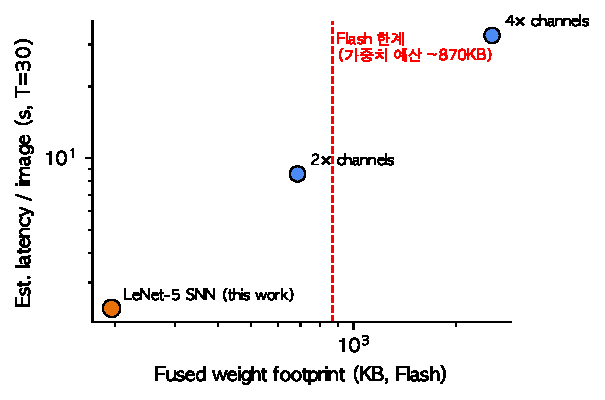
\includegraphics[width=0.86\linewidth]{figures/fig_envelope.pdf}
\caption{배포 가능 영역: 퓨전 가중치 Flash 용량 대 이미지당 추정
지연($T=30$, 양 축 로그). 수직 점선은 가중치 예산 약 870KB($=$1MB
$-$ 코드$\cdot$런타임 178.5KB)이며, 현 모델은 실측점,
2$\times$/4$\times$ 구성은 추정점이다.}
\label{fig:envelope}
\end{figure}

\subsection{타임스텝 축소 축}

지연의 또 다른 축은 $T$이다. 타임스텝당 시간이 일정하므로 지연은
$T$에 선형이고, $T=30\rightarrow10$이면 이미지당 약 0.8초로 추정된다.
학습 단계에서 관찰한 단일 이미지의 누적 스파이크 수렴 곡선은 판정이
$T<30$에서 조기 수렴할 수 있음을 시사하나, 이는 정성적 예시일 뿐이며
$T$ 축소에 따른 정확도 트레이드오프는 본 논문에서 검증하지 않았다.


\section{결론 및 향후 연구}
\label{sec:conclusion}

본 논문은 NPU가 없는 초소형 MCU(STM32F746, SRAM 320KB, Flash
1MB)에서 QAT로 학습된 SNN을 정수 전용 코드로 lowering하는
CHACHA 컴파일러와, Conv+AvgPool+LIF를 하나로 묶은 TFLM 커스텀 연산자를
제시하였다. 표준 TFLM+CMSIS-NN 경로가 s16 DSP fast 경로의 커버리지
제약으로 스칼라 구현보다 약 2.1배 느려지는 성능 역전을 실측으로
규명하였고, 제안 퓨전 연산자가 이를 동일 조건 4.0배 가속(이미지당
$2{,}407$ms, 타임스텝당 77.9ms, 아레나 실사용 80.3KB)으로 회복함을
보였다. TFLM 런타임 오버헤드는 약 0.5\%로 무시 가능함을 분리
실측하였으며, 호스트 비트 일치 검증과 LIF SIMD 전수 검증으로 구현의
비트 정확성을 확인하였다. 나아가 메모리 비용 모델과 실측 처리량으로
배포 가능 영역을 정량화하여, 현 보드에서 채널 2배 구성까지 배포
가능(추정)하고 4배 구성은 Flash 초과로 불가함을 제시하였다.

향후 과제는 다음과 같다. (1) 다중 모델$\cdot$다중 데이터셋으로의 검증
확대, (2) 정수 구현의 전체 테스트셋 정확도 실측, (3) 출력 채널 타일
제약($C_o\le64$)의 완화, (4) 타임스텝 축소와 조기 판정에 따른
지연--정확도 트레이드오프 탐색, (5) 전력 실측과 스파이크 희소성을
활용하는 zero-skipping 커널 --- 본 구현은 희소성을 활용하지 않는
dense 연산이며 에너지 실측도 수행하지 않았다 ---, (6)
NIR\cite{pedersen2024nir}와 같은 SNN 교환 포맷으로부터의 임포트
연계이다. 현 컴파일러의 입력은 snnTorch+Brevitas 그래프에 한정되므로,
교환 포맷 연계는 적용 범위를 넓히는 다음 단계가 될 것이다.


\bibliographystyle{ieeetr}
{\footnotesize
\bibliography{references}
}

\end{document}
